\chapter{二次曲线}
\begin{proverb}
  { \itshape
   It is easy to teach someone, but to show him
   an easy way to realize the learned things, this
   is something to admire.
  }

\hfill St. John Chrysostom(347--407)
\end{proverb}

\section{二次曲线}
\begin{definition}
  代数平面曲线是其隐式方程为下列形式的曲线
  \[
    \mathscr C:\quad F(x,y) = 0,
  \]
  其中$F$是一个关于变量$x$和$y$的多项式. 多项式的次数称为代数曲线的次数.
\end{definition}

\begin{definition}
  二次曲线是次数为2的代数曲线. 二次曲线的一般方程为
  \[
    \mathscr C:\quad a_{11}x^2 + 2a_{12}xy + a_{22}y^2 + b_1x + b_2y + c = 0,
  \]
  其中$a_{11},a_{12},a_{22},b_1,b_2,c\in\MR$且$a_{11}^2+a_{12}^2
  +a_{22}^2\ne0$.
\end{definition}

当特殊选取平面坐标系的时候,二次曲线会有一个简单的形式,称为标准形. 我们回顾非退化的二次曲线.

{\noindent \kaishu 非退化的二次曲线}

\begin{itemize} \parindent=2em
  \item {\bfseries 椭圆} 定义成平面上到两个不同点$F(c,0)$和$F'(-c,0)$的距离之和为常数的点$M(x,y)$的集合,其中常数$c>0$称为{\kaishu 焦距}. 因此,满足性质$MF+MF'=2a.a>c$的点$M(x,y)$构成的集合$\mathscr E$叫做椭圆(图 \ref{fig6.1}).
      \begin{figure}[!ht]
        \centering
          \begin{tikzpicture}
    \draw [->] (-4,0) -- (-3,0) node[below left]
    {$A'$} -- (-2.236,0)node[below] {$F'$} -- (0,0)
    node[below left] {$O$} -- (2.236,0)node[below]
    {$F$} -- (3,0) node[below right] {$A$} -- (4,0)
    node[below] {$x$};
    \draw [->] (0,-3) -- (0,-2) node[below left]
    {$B'$} -- (0,2) node[above left]{$B$} -- (0,3)
    node[left] {$y$};
    \draw [domain=0:360,blue]
    plot({3*cos(\x)},{2*sin(\x)});
    \draw [red!70!black] (-2,0) --
    ({3*cos(60)},{2*sin(60)})node[above,black]{$M$}
    ({3*cos(60)},{2*sin(60)}) -- (2,0);
  \end{tikzpicture}

        \caption{椭圆$\frac{x^2}{a^2}+\frac{y^2}{b^2}=1,a,b>0$}\label{fig6.1}
      \end{figure}

      设$b^2=a^2-c^2$. 椭圆的方程为
      \begin{align*}
        & \mathscr E:\quad \frac{x^2}{a^2} + \frac{y^2}{b^2} = 1\quad \text{直接方程} \\
        & \mathscr E:\quad \left\{
           \begin{aligned}
             & y = \frac ba \sqrt{a^2 - x^2} \\
             & y = -\frac ba \sqrt{a^2 - x^2}
           \end{aligned}
           \right.,x\in[-a,a]\quad \text{笛卡尔方程} \\
        & \mathscr E:\quad \left\{
            \begin{aligned}
              & x = a\cos t \\
              & y = b\sin t
            \end{aligned}
          \right.,t\in[0,2\pi) \quad \text{参数方程}
      \end{align*}

     当$a=b=r$时,椭圆变成圆
     \[
       x^2 + y^2 = r^2 \quad \text{或} \quad
       \left\{
         \begin{aligned}
           & x = r \cos t \\
           & y = r \sin t
         \end{aligned}
       \right.,\quad t\in[0,2\pi).
     \]
     {\kaishu 光学性质.} 椭圆上一点的切线和法线是由{\kaishu 焦半径}确定的角的平分线.
  \item {\bfseries 双曲线} 定义成平面上到两个不同点$F(c,0)$和$F'(-c,0)$的距离之差的绝对值为常数的点$M(x,y)$的集合,其中常数$c>0$称为{\kaishu 焦距}. 因此,满足性质$|MF-MF'|=2a,0<a<c$的点$M(x,y)$的集合$\mathscr H$称为是双曲线(图 \ref{fig6.2}).
      \begin{figure}[!ht]
        \centering
          \begin{tikzpicture}
    \draw [->] (-6,0) -- (-3,0) node[below] {$F'$} -- (-2.236,0) node[below right] {$A'$} -- (0,0) node[below left] {$O$} -- (2.236,0) node[below left]{$A$} -- (3,0) node[below] {$F$} -- (6,0) node [below] {$x$};
    \draw [->] (0,-4) -- (0,4) node[left] {$y$};
    \draw [thick,blue,domain = -60:60] plot ({2.236*sec(\x)},{2*tan(\x)});
    \draw [thick,blue,xscale=-1, domain = -60:60] plot ({2.236*sec(\x)},{2*tan(\x)});
    \draw [blue!70!cyan,domain=-4:4] plot (\x,{2*\x/2.236}) node [above,black]{$y=\frac bax$};
    \draw [blue!70!cyan,domain=4:-4] plot (\x,{-2*\x/2.236})node [above,black]{$y=-\frac bax$};
    \draw [red!50!black] (-3,0) -- ({2.236*sec(45)},{2*tan(45)}) node[right,black]{$M$} -- (3,0);
  \end{tikzpicture}
        \caption{双曲线$\frac{x^2}{a^2}-\frac{y^2}{b^2}=1,a,b>0$}\label{fig6.2}
      \end{figure}

      由$F$和$F'$确定直线称为{\kaishu 焦轴},线段$FF'=2c$称为{\kaishu 焦距},线段$MF$和$MF'$称为{\kaishu 焦半径}. 直接计算可得双曲线的方程为:
      \begin{align*}
        & \mathscr H:\quad \frac{x^2}{a^2} - \frac{y^2}{b^2} = 1\quad \text{直接方程} \\
        & \mathscr H:\quad \left\{
           \begin{aligned}
             & y = \frac ba \sqrt{x^2 - a^2} \\
             & y = -\frac ba \sqrt{x^2 - a^2}
           \end{aligned}
           \right.,x\in(-\infty,-a]\cup[a,+\infty)\quad \text{笛卡尔方程} \\
        & \mathscr H:\quad \left\{
            \begin{aligned}
              & x = \pm a\cosh t \\
              & y = b\sinh t
            \end{aligned}
          \right.,t\in\MR \quad \text{参数方程}
      \end{align*}
      其中
      \[
        \cosh t = \frac{\ee^t + \ee^{-t}}2 \quad \text{且} \quad
        \sinh t = \frac{\ee^t - \ee^{-t}}2.
      \]
      双曲线是一个无界的曲线,其渐近线为$y=\frac bax$和$y=-\frac bax$. 渐近线互相正交的双曲线称为是等轴的.

      {\kaishu 光学性质.} 双曲线上一点的切线和法线是由焦半径确定的角的平分线.

    \item {\bfseries 抛物线} 定义成平面上到一个定直线$x=-\frac p2,p>0$和一个定点$F\left(\frac p2,0\right)$的距离相等的点$M(x,y)$的集合,其中定直线称为{\kaishu 准线},定点称为{\kaishu 焦点}(图 \ref{fig6.3}).
        \begin{figure}[!ht]
          \centering
            \begin{tikzpicture}[yscale = 0.8]
    \draw [->] (-2,0) -- (-1,0) node[below left] {$A$} -- (0,0) node[below left] {$O$} -- (1,0) node[below] {$F$} -- (5,0) node[below] {$x$};
    \draw [->] (0,-4) -- (0,4) node [left]{$y$};
    \draw [domain=-4:4,blue!60!black,semithick] plot (\x*\x/4,\x);
    \draw [blue!70!cyan] (-1,-4)node[above left,black] {$x=-\frac p2$} -- (-1,4);
    \draw [red!60!black](-1,2.8) node [left,black] {$B$} -- (1.96,2.8)node[above,black]{$M$} -- (1,0);
  \end{tikzpicture}
          \caption{抛物线$y^2=2px,p>0$}\label{fig6.3}
        \end{figure}

        因此,抛物线的方程为
        \begin{align*}
          & \mathscr P:\quad y^2 = 2px \quad \text{直接方程} \\
          & \mathscr P:\quad
            \left\{
              \begin{aligned}
                & x = \frac{t^2}{2p} \\
                & y = t
              \end{aligned}, t \in \MR\quad \text{参数方程}
            \right.
        \end{align*}
      一般地,抛物线也被定义成其函数图像具有以下形式:
      \[
        y = ax^2 + bx +c ,a\ne 0 \quad \text{或}\quad x = a'y^2 + b'y + c',a'\ne0.
      \]
      {\kaishu 光学性质.} 抛物线上一点的切线和法线是由焦点半径和通过该点到抛物线轴线的平行线确定的角的平分线.
\end{itemize}

{\noindent\kaishu 退化的二次曲线 }

二次代数曲线中退化的二次曲线为:
\begin{itemize}
  \item $\mathscr C:(a_1x+b_1y+c_1)(a_2x+b_2y+c_2)=0$(两条直线的并);
  \item $\mathscr C:\alpha(x-x_0)^2+\beta(y-y_0)^2=0,\alpha,
      \beta>0$(一个点);
  \item $\mathscr C:\alpha(x-x_0)^2+\beta(y-y_0)^2+\delta=0,
      \alpha,\beta,\delta>0$(空集).
\end{itemize}

利用初等几何可以得出二次曲线的基本性质,见 \cite{2}.

\section{化二次曲线为标准形}
设
\begin{equation}\label{eq6.1}
  \mathscr C:\quad a_{11}x^2 + 2a_{12}xy + a_{22}y^2 + b_1x + b_2y + c = 0,
\end{equation}
是在$xOy$面上的一个二次曲线,其中$a_{11},a_{12},a_{22},b_1,b_2,c\in\MR$且
$a_{11}^2+a_{12}^2+a_{22}^2\ne0$.

要将一个二次曲线化为其标准形,我们要在平面上选取一个坐标系,使得在新的坐标系下,二次曲线有一个简单的方程.,即所谓的约化方程. 我们将看到,任意一个这样的坐标变换由两个几何变换,即一个平移和一个旋转构成(和最后一个经过坐标轴的反射). 这些变换是基于二阶对称矩阵的Jordan标准形来决定的.

设$f(x,y)=a_{11}x^2+2a_{12}xy+a_{22}y^2$是方程 \eqref{eq6.1} 中的二次项部分,而$A_f$是$f$对应的对称矩阵
\[
  A_f = \begin{pmatrix}
    a_{11} & a_{12} \\
    a_{12} & a_{22}
  \end{pmatrix}.
\]
\begin{nota}
  在矩阵$A_f$的副对角线上的系数等于二次曲线中$xy$的系数的一半.
\end{nota}

熟知(定理 \ref{thm2.5})矩阵$A_f$是可对角化的,且可以取矩阵$P\in\MM_2(\MR)$是一个正交矩阵,即$P\TT=P^{-1}$. 事实上,$P$是一个旋转矩阵. $A_f$的特征值是实数$\lambda_1,\lambda_2$(见定理 \ref{thm2.5}),且其中至少有一个是非零的,因为$A_f\ne O_2$.

设
\[
  J_{A_f} = \begin{pmatrix}
    \lambda_1 & 0 \\
    0 & \lambda_2
  \end{pmatrix} = P\TT A_fP,
\]
其中$P$是由相应于特征值$\lambda_1$和$\lambda_2$的单位特征向量构成的矩阵.

{\bfseries 旋转.} 我们通过在$xOy$平面上进行正交变换来改变坐标系,由矩阵$P$定义的旋转为
\[
  \begin{pmatrix}
    x \\
    y
  \end{pmatrix} = P
  \begin{pmatrix}
    x' \\
    y'
  \end{pmatrix},
\]
则坐标系$xOy$变为$x'Oy'$.

利用公式
\[
  [f(x,y)] = \begin{pmatrix}
    x \\
    y
  \end{pmatrix}\TT A_f \begin{pmatrix}
    x \\
    y
  \end{pmatrix},
\]
我们得到
\[
  [f(x,y)] = \left( P\begin{pmatrix}
    x' \\
    y'
  \end{pmatrix} \right)\TT A_f P
  \begin{pmatrix}
    x' \\
    y'
  \end{pmatrix} =
  \begin{pmatrix}
    x' \\
    y'
  \end{pmatrix}\TT J_{A_f}
  \begin{pmatrix}
    x' \\
    y'
  \end{pmatrix} =
  \lambda_1x'^2 + \lambda_2y'^2.
\]
因此,在新坐标系$x'Oy'$下,二次曲线的方程变为
\begin{equation}\label{eq6.2}
  \mathscr C:\quad \lambda_1 x'^2 + \lambda_2y'^2 + b_1'x' + b_2'y' + c = 0,
\end{equation}
其中系数$b_1',b_2'$由公式
\[
  b_1x + b_2y = b_1'x' + b_2'y'\quad \Leftrightarrow
  \quad [b_1\,b_2]\begin{pmatrix}
    x \\
    y
  \end{pmatrix} = [b_1'\,b_2']
  \begin{pmatrix}
    x' \\
    y'
  \end{pmatrix}
\]
所决定,这等价于
\[
  [b_1\,b_2] P \begin{pmatrix}
    x' \\
    y'
  \end{pmatrix} =
  [b_1'\,b_2'] \begin{pmatrix}
    x' \\
    y'
  \end{pmatrix}, \quad \text{所以} \quad
  [b_1'\,b_2'] = [b_1\,b_2]P.
\]

\begin{nota}
  旋转的目的是使得$xy$的项消失.
\end{nota}

{\bfseries 平移.} 我们分$A_f$是特征值都非零和其中有一个为零的两种情形.

{\kaishu 情形1.} 如果$\lambda_1\ne0$且$\lambda_2\ne0$,我们将方程 \eqref{eq6.2} 写成
\[
  \mathscr C :\quad \lambda_1\left( x' + \frac{b_1'}{2\lambda_1} \right)^2 + \lambda_2
  \left( y' + \frac{b_2'}{2\lambda_2} \right)^2 + c' = 0,
\]
其中
\[
  c' = c - \frac{b_1'^2}{4\lambda_1} - \frac{b_2'^2}{4\lambda_2}.
\]

现在我们平移坐标系$x'Oy'$到坐标系$x''O''y''$,平移公式为
\[
  T:\left\{
    \begin{aligned}
      & x'' = x' + \frac{b_1'}{2\lambda_1} \\
      & y'' = y' + \frac{b_2'}{2\lambda_2}
    \end{aligned}
  \right..
\]

新坐标系的中心为$O''$,其坐标满足
\[
  x'' = y'' =0 \quad \Leftrightarrow \quad
  x' = - \frac{b_1'}{2\lambda_1},y' = - \frac{b_2'}{2\lambda_2} \quad \Leftrightarrow \quad
  \begin{pmatrix}
    x \\
    y
  \end{pmatrix} = P
  \begin{pmatrix}
    x' \\
    y'
  \end{pmatrix}.
\]
二次曲线的方程变为
\[
  \mathscr C:\quad \lambda_1x''^2 + \lambda_2y''^2 + c' = 0.
\]

如果$c'=0$,我们得到一个退化的二次曲线,它是一个点或两条直线的并.

如果$c'\ne0$,二次曲线或者是椭圆,或者是双曲线,取决于特征值$\lambda_1,\lambda_2$是否具有相同的符号.

{\bfseries 情形2.} 如果其中一个特征值为0,不妨设$\lambda_2=0$
且$\lambda_1\ne0$,我们有
\[
  \mathscr C: \quad \lambda_1 \left( x' + \frac{b_1'}{2\lambda_1} \right)^2 + b_2'y' + c' = 0,\quad c' = c - \frac{b_1'^2}{4\lambda_1},
\]
在这种情形下, 平移公式为
\[
  T: \left\{
    \begin{aligned}
      & x'' = x' + \frac{b_1'}{2\lambda_1} \\
      & y'' = y' + \frac{c'}{b_2'}
    \end{aligned}
  \right..
\]
此二次曲线是一个抛物线,其方程为
\[
  \mathscr C:\quad \lambda_1x''^2 + b_2'y'' = 0.
\]
\begin{nota}
  平移公式是在完成对$x'$或$y'$的配方之后所决定的.
\end{nota}

\begin{remark}
  如果二次曲线是非退化的,则其类型只需要通过分析$A_f$的特征值的符号即可得到. 确切地讲,如果

  $\lambda_1\lambda_2>0$,则二次曲线为椭圆;

  $\lambda_1\lambda_2<0$,则二次曲线为双曲线;

  $\lambda_1\lambda_2=0$,则二次曲线为抛物线.
\end{remark}

现在我们总结上面使用的技巧,并给出一个化二次曲线为标准形的算法.

\begin{mybox}
  {\bfseries 化二次型为标准形的算法}

  \begin{itemize}
    \item {\bfseries 步骤1.} 写出矩阵$A_f$并求出其特征值.
    \item {\bfseries 步骤2.} 求出Jordan标准形$J_{A_f}$和正交矩阵$P,P\TT=P^{-1}$,其满足等式
        \[
          J_{A_f} = \begin{pmatrix}
            \lambda_1 & 0 \\
            0 & \lambda_2
          \end{pmatrix} = P\TT A_fP.
        \]
    \item {\bfseries 步骤3.} 将旋转公式写成
        \[
          X = PY,\quad \text{其中} \quad
          X = \begin{pmatrix}
            x \\
            y
          \end{pmatrix} \quad \text{且} \quad
          Y = \begin{pmatrix}
            x' \\
            y'
          \end{pmatrix}.
        \]
        写出$P=R_\alpha$,求出旋转角. 因此,坐标系$xOy$逆时针旋转角度$\alpha$变成了坐标系$x'Oy'$.
    \item {\bfseries 步骤4.} 对$x'$或$y'$完成配方以后写出平移公式.
    \item {\bfseries 步骤5.} 分析关于$x''$和$y''$的方程来确定二次曲线的类型.
  \end{itemize}
\end{mybox}

\begin{example}
  {\bfseries 双曲线.} 我们考虑二次曲线
  \[
    \mathscr C: \quad 3x^2 + 10xy + 3y^2 - 2x - 14y - 13 = 0,
  \]
  我们将其化为标准形,并决定其类型(图 \ref{fig6.4}).
\end{example}
\begin{figure}[!ht]
  \centering
  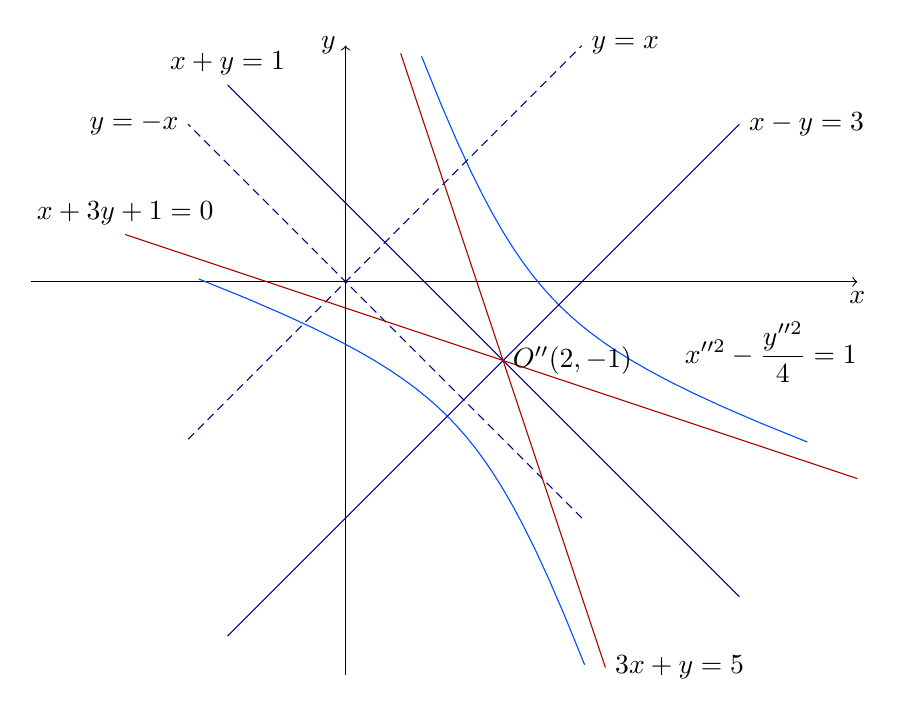
\begin{tikzpicture}[every node/.style={black}]
  \draw [->] (-4,0) -- (6.5,0) node [below] {$x$};
  \draw [->] (0,-5) -- (0,3) node [left] {$y$};
  \begin{scope}[shift = {(2,-1)},blue!70!cyan]
    \draw [rotate = 45,domain=-60:60] plot ({sec(\x)},{2*tan(\x)});
    \draw [rotate = 45,domain=-60:60] plot ({-sec(\x)},{2*tan(\x)});
  \end{scope}
  \draw [blue!50!black] plot[domain=-1.5:5] (\x,\x-3) node[right] {$x-y=3$}
  plot[domain = 5:-1.5] (\x,1-\x)node[above] {$x+y=1$};
  \draw [densely dashed,blue!50!black,domain = -2:3] plot[domain = 3:-2] (\x,-\x)node[left] {$y=-x$} plot(\x,\x) node[right]{$y=x$};
  \draw [red!70!black] plot [domain = -2.5:0.6] (-3*\x-1,\x) node[above] {$x+3y+1=0$}
  plot [domain = 0.7:3.3] (\x,5-3*\x) node [right]{$3x+y=5$};
  \node at (5.4,-0.9) {$\displaystyle x''^2-\frac{y''^2}4=1$};
  \node [right] at (2,-1) {$O''(2,-1)$};
\end{tikzpicture} 
  \caption{双曲线$3x^2+10xy+3y^2-2x-14y-13=0$}\label{fig6.4}
\end{figure}

{\bfseries 步骤1.} 与二次曲线对应的二次型为$f(x,y)=3x^2+10xy+3y^2$,其相应的对称矩阵为
\[
  A_f = \begin{pmatrix}
    3 & 5 \\
    5 & 3
  \end{pmatrix}.
\]

$A_f$的特征值通过解方程$\det(A_f-\lambda I_2)=0$得到,这意味着$(3-\lambda)^2-25=0\Rightarrow\lambda_1=8,\lambda_2=-2$.

{\bfseries 步骤2.} 我们求出相应于特征值$\lambda_1=8$和$\lambda_2=-2$的特征向量. 相应于特征值$\lambda_1=8$的特征向量要解方程$(A_f-8I_2)X=0$,我们有
\[
  \left\{
    \begin{aligned}
      & -5x_1 + 5x_2 = 0 \\
      & 5x_1 - 5x_2 = 0
    \end{aligned}
  \right.,
\]
这意味着$x_1=x_2$,方程组的解为$\begin{pmatrix}
  \alpha \\
  \alpha
\end{pmatrix},\alpha\in\MR^\ast$. 我们设$\alpha=1$,并将这里的向量除以它的范数(长度),我们得到特征向量
\[
  X_1 = \begin{pmatrix}
    \frac1{\sqrt2} \\
    \frac1{\sqrt2}
  \end{pmatrix}.
\]

类似地,相应于$\lambda_2=-2$的特征向量要解方程组$(A_f+2I_2)X=0$,我们得到特征向量
\[
  X_2 = \begin{pmatrix}
    -\frac1{\sqrt2} \\
    \frac1{\sqrt2}
  \end{pmatrix}.
\]

因此,
\[
  P = \begin{pmatrix}
    \frac1{\sqrt2} & - \frac1{\sqrt2} \\
    \frac1{\sqrt2} & \frac1{\sqrt2}
  \end{pmatrix} =
  \begin{pmatrix}
    \cos\frac\pi4 & - \sin\frac\pi4 \\
    \sin\frac\pi4 & \cos \frac\pi4
  \end{pmatrix} = R_{\frac\pi4},
\]
这是角度为$\frac\pi4$的旋转矩阵.

{\bfseries 步骤3.} 旋转公式为
\begin{equation}\label{eq6.3}
  \begin{pmatrix}
    x \\
    y
  \end{pmatrix} = P
  \begin{pmatrix}
    x' \\
    y'
  \end{pmatrix} \quad \text{或} \quad
  \left\{
    \begin{aligned}
      & x = \frac1{\sqrt2}x' - \frac1{\sqrt2}y' \\
      & y = \frac1{\sqrt2}x' + \frac1{\sqrt2}y'
    \end{aligned}
  \right..
\end{equation}

我们将坐标系$xOy$逆时针旋转角度$\frac\pi4$,则二次曲线的方程变为
\[
  \mathscr C;\quad 8x'^2 - 2y'^2 - \frac2{\sqrt2}(x' - y') - \frac{14}{\sqrt2}(x' + y') - 13 = 0,
\]

{\bfseries 步骤4.}  平移公式为
\[
  T: \left\{
    \begin{aligned}
      & x'' = x - \frac1{\sqrt2} \\
      & y'' = y' + \frac3{\sqrt2}
    \end{aligned}
  \right..
\]
因此,我们将坐标系$x'Oy'$平移到$x''O''y''$,二次曲线的方程变为
\[
  \mathscr C:\quad 8x''^2 - 2y''^2 - 8 = 0 \quad \Leftrightarrow \quad x''^2 - \frac{y''^2}4 = 1.
\]
于是,我们二次曲线是一个双曲线,半轴长分别为$a=1$和$b=2$.

接下来,我们求出方程的对称轴和坐标系的中心$O'$.

由 \eqref{eq6.3},我们有$\begin{pmatrix}
  x' \\
  y'
\end{pmatrix}=P^{-1}\begin{pmatrix}
  x \\
  y
\end{pmatrix}=P\TT\begin{pmatrix}
  x \\
  y
\end{pmatrix}$,而这意味着
\begin{equation}\label{eq6.4}
  \left\{
    \begin{aligned}
      & x' = \frac1{\sqrt2} (x + y) \\
      & y' = \frac1{\sqrt2} (-x + y)
    \end{aligned}
  \right..
\end{equation}

{\kaishu $O''x''$的方程.} 要求出$O''x''$的方程,我们令$y''=0$,这反过来说明$y'=-\frac3{\sqrt2}$. \eqref{eq6.4} 的第二个方程说明$-x+y=-3$.

{\kaishu $O''y''$的方程.}  要求出$O''y''$的方程,我们令$x''=0$,这意味着$x'=\frac1{\sqrt2}$. 然而, \eqref{eq6.4} 中的第一个方程意味着$x+y=1$.

{\kaishu 对称中心$O''$的坐标.} $O''$的坐标是方程组
\[
  \left\{
    \begin{aligned}
      & x + y = 1\\
      & -x + y = -3
    \end{aligned}
  \right.
\]
的解,这说明$x=2,y=-1$. 因此,$O''(2,-1)$,即$O''$在坐标系$xOy$下的坐标为$(2,-1)$.

\section{问题}
\begin{problem}
  求出下面二次曲线的标准形,判断其类型,求出对称轴及其中心:
  \begin{enumerate}[left=0cm,align=right,label=(\arabic*)]
    \item $3x^2-4xy+3y^2-2x-2y+1=0$;
    \item $2x^2-4xy-y^2+\sqrt5x+\sqrt5y-1=0$;
    \item $x^2-2xy+y^2+2x-4y+5=0$;
    \item $4x^2+12xy+9y^2-64=0$;
    \item $9x^2+24xy+16y^2-40x+30y=0$;
    \item $2x^2-6xy+10y^2-8x+12y+2=0$;
    \item $4x^2-4xy+y^2-2x-14y+7=0$;
    \item $4xy-3y^2+4x-14y-7=0$;
    \item $3x^2-4xy-2x+4y-3=0$;
    \item $x^2+2xy+y^2+2x+2y-3=0$;
    \item $x^2-8xy+7y^2+6x-6y+9=0$;
    \item $5x^2+12xy-22x-12y-19=0$;
    \item $6x^2-4xy+9y^2-4x-32y-6=0$;
    \item $5x^2+4xy+8y^2-32x-56y+80=0$;
    \item $xy-k=0,k\in\MR^\ast$.
  \end{enumerate}
\end{problem}

\begin{problem}
  根据参数$a$的值,讨论下列二次曲线的类型:
  \begin{enumerate}[left=0cm,align=right,label=(\arabic*)]
    \item $5x^2+2axy+5y^2+2x+2y+2=0$;
    \item $ax^2+2xy+ay^2-2x+2y+9=0$;
    \item $x^2+4xy+4y^2+ax=0$;
    \item $7x^2-8xy+y^2+a=0$.
  \end{enumerate}
\end{problem}

\begin{problem}
  对怎样的$c$,笛卡尔方程$2xy-4x+6y+c=0$表示一对直线?
\end{problem}

\begin{problem}
  {\kaishu 等轴双曲线.} 证明:二次曲线$(x+2y+1)(2x-y+1)+\alpha=0,\alpha\ne0$是一个双曲线,且其渐近线为$x+2y+1=0$和$2x-y+1=0$.
\end{problem}

\begin{remark}
  更一般地,我们可以证明二次曲线
  \[
    (a_1x + b_1y + c_1)(a_2x + b_2y + c_2) + \alpha = 0,a_1b_2 - a_2b_1\ne0,\alpha\ne0
  \]
  是一个双曲线,且其渐近线为$a_1x+b_1y+c_1=0$和$a_2x+b_2y+c_2=0$.
\end{remark}

\begin{problem}
  \begin{inparaenum}[(a)]
    \item 求出经过点$(1,1),(2,1)$和$(-1,-2)$,且以$x+y-1=0$为渐近线的双曲线的方程.

    \item 求出过点$(1,1)$和$(2,1)$,且以$x-y+1=0$为渐近线的等轴双曲线的方程.
  \end{inparaenum}
\end{problem}

\begin{mybox}
  \begin{problem}[一个Lam\'e曲线和一个伪装的抛物线.]
  
    设实数$k>0$,证明曲线:$\mathscr C_k^1:\sqrt y - \sqrt x = \sqrt k,\mathscr C_k^2:\sqrt x+\sqrt y=\sqrt k$和$\mathscr C_k^3:\sqrt x-\sqrt y=\sqrt k$合起来构成了一个抛物线,求出其标准形,顶点和对称轴.
  \end{problem}
\end{mybox}

\begin{remark}
  一个{\kaishu Lam\'e曲线}\index{L!Lam\'e曲线}的笛卡尔方程为$\frac{x^\alpha}{a^\alpha}+\frac{y^\alpha}{b^\alpha}=1$,其中$a,b$是正实数,而$\alpha$为实数. 这类曲线被G.Lam\'e \cite{39} 在19世纪所研究,现在它们被称为{\kaishu Lam\'e曲线}或{\kaishu 超椭圆}.

  当$k=1$时,曲线$\mathscr C_1^2$在 \cite{12} 中讨论了,它说明虽然$\mathscr C_1^2$看起来像是圆弧,但实际上$\mathscr C_1^2$是双曲线的一部分.
\end{remark}

\begin{problem}
  求出二次曲线$\mathscr C:x^2+y^2-4xy-1=0$的类型,并求出$\mathscr C$上的格点.
\end{problem}

\begin{problem}
  证明双曲线$\mathscr H$:$x^2-5y^2=4$包含无穷多个格点.
\end{problem}

\begin{problem}
  \begin{inparaenum}[(a)]
    \item\label{prob6.9a} 求出$xOy$平面上的一个椭圆,其焦点为$F_1(\sqrt3,2),F_2(3\sqrt3,4)$,且长半轴为$a=3$.

    \item 求出 (\ref{prob6.9a}) 中二次曲线的标准形.
  \end{inparaenum}
\end{problem}

\begin{problem}
  \begin{inparaenum}[(a)]
    \item\label{prob6.10a} 求出焦点为$F_1(-1,2),F_2(3,6)$,半轴为$a=2$的双曲线方程.

    \item 求出 (\ref{prob6.10a}) 中二次曲线的标准形.
  \end{inparaenum}
\end{problem}

\begin{problem}
  \begin{inparaenum}[(a)]
    \item\label{prob6.11a} 求出$xOy$平面上到直线$\mathscr D:\sqrt3x-3y+2\sqrt3=0$和到点$F(2,0)$距离相等的点$M(x,y)$的轨迹.

    \item 求出 (\ref{prob6.11a}) 中二次曲线的标准形.
  \end{inparaenum}
\end{problem}

\begin{problem}[\kaishu 由椭圆决定的Abel群.]

设$\mathscr E$表示椭圆$\frac{x^2}{a^2}+\frac{y^2}{b^2}=1$,且设$\ast$是一个作用于$\mathscr E$的二元算符,其定义为$\ast:\mathscr E\times\mathscr E\to\mathscr E,(M_1,M_2)\in\mathscr E\times\mathscr E\to
M_1\ast M_1\in\mathscr E$,其中$M_1\ast M_2$是过点$A(a,0)$且平行于线段$[M_1M_2]$的直线与椭圆$\mathscr E$的交点. 证明$(\mathscr E,\ast)$是一个Abel群.
\end{problem}

\begin{problem}
  求函数$f(x,y)=x^2+xy+y^2+x-y-1$的最值以及对应的极值点.
\end{problem}

\begin{problem}[\kaishu 带限制条件的极值问题.]

  \begin{inparaenum}[(a)]
    \item 求函数$f(x,y)=x+y$在条件$3x^2-2xy+3y^2+4x+4y-4=0$下的最大值和最小值.

    \item 求函数$f(x,y)=2x+y$在条件$3x^2+10xy+3y^2-16x-16y-16=0$下的极值.

    \item 求函数$f(x,y)=2x-y$在条件$9x^2+24xy+16y^2-40x+30y=0$下的极值.
  \end{inparaenum}
\end{problem}

\begin{mybox}
  \begin{problem}[一个二次型的条件极值.]

    设函数$f(x,y)=ax^2+2bxy+cy^2,a,b,c\in\MR$满足$a^2+b^2+c^2\ne0$. 证明:函数$f$在条件$x^2+y^2=1$下的最小值和最大值分别是矩阵
    \[
      A_f = \begin{pmatrix}
        a & b \\
        b & c
      \end{pmatrix}
    \]
    的最小和最大特征值.
  \end{problem}
\end{mybox}

\begin{problem}
  求出由曲线
  \[
    5x^2 + 6xy + 5y^2 - 16x - 16y - 16 = 0
  \]
  所围成区域的面积.
\end{problem}

{\noindent \kaishu 椭圆域上的二重积分.}

\begin{problem}
  计算:
  \begin{enum}
    \item $\iint_{D_1}\ee^{x^2-xy+y^2}\dif x\dif y$,其中$D_1=\{(x,y)\in\MR^2:x^2-xy+y^2\le1\}$;
    \item $\iint_{D_2}\ee^{x^2+xy+y^2}\dif x\dif y$,其中$D_2=\{(x,y)\in\MR^2:x^2+xy+y^2\le1\}$;
    \item $\iint_{D_3}\ee^{-x^2+xy-y^2}\dif x\dif y$,其中$D_3=\{(x,y)\in\MR^2:x^2-xy+y^2\ge1\}$;
    \item $\iint_{D_4}\ee^{-x^2-xy-y^2}\dif x\dif y$,其中$D_4=\{(x,y)\in\MR^2:x^2+xy+y^2\ge1\}$.
  \end{enum}
\end{problem}

\begin{problem}
  设$a,b\in\MR$满足$0<b<2a$,且设$\alpha>0$. 计算:
  \begin{enum}
    \item $\iint_{D_1}\ee^{ax^2-bxy+ay^2}\dif x\dif y$,其中$D_1=\{(x,y)\in\MR^2:ax^2-bxy+ay^2\le\alpha\}$;
    \item $\iint_{D_2}\ee^{ax^2+bxy+ay^2}\dif x\dif y$,其中$D_2=\{(x,y)\in\MR^2:ax^2+bxy+ay^2\le\alpha\}$;
    \item $\iint_{D_3}\ee^{-ax^2+bxy-ay^2}\dif x\dif y$,其中$D_3=\{(x,y)\in\MR^2:ax^2-bxy+ay^2\ge\alpha\}$;
    \item $\iint_{D_3}\ee^{-ax^2-bxy-ay^2}\dif x\dif y$,其中$D_4=\{(x,y)\in\MR^2:ax^2+bxy+ay^2\ge\alpha\}$.
  \end{enum}
\end{problem}

\begin{mybox}
  \begin{problem}
    设$ab\in\MR$满足$0<b<2a$,且设$\alpha>0$. 计算:
    \begin{enum}
      \item \label{prob6.19a} $\iint_{D_\alpha}x\ee^{-ax^2-bxy-ay^2}\dif x\dif y$;
      \item \label{prob6.19b} $\iint_{D_\alpha}xy\ee^{-ax^2-bxy-ay^2}\dif x\dif y$,
    \end{enum}
    其中$D_\alpha=\{(x,y)\in\MR^2,ax^2+bxy+ay^2\ge\alpha\}$.
  \end{problem}
\end{mybox}

\begin{mybox}
  \begin{problem}[二次型和特殊积分.]

    \begin{inparaenum}[(a)]
      \item 计算
      \[
        \iint_{\MR^2} \frac{\dif x\dif y}{(1+3x^2-4xy+3y^2)^3}.
      \]

      \item 设$A\in\MM_2(\MR)$是一个具有正特征值的对称矩阵,且设实数$\alpha>1$. 证明:
      \[
        \iint_{\MR^2} \frac{\dif x\dif y}{(1+v\TT Av)^\alpha} = \frac\pi{(\alpha-1)\sqrt{\det A}},\quad \text{其中} \quad v = \begin{pmatrix}
          x \\
          y
        \end{pmatrix}.
      \]

      \item 设$f$是$[0,+\infty)$上的一个可积函数,且设$\int_0^{+\infty}f(x)\dif x=I$. 证明:如果$A\in\MM_2(\MR)$是一个具有正特征值的对称矩阵,则
          \[
            \iint_{\MR^2}f\left( v\TT Av \right) =
            \frac{\pi I}{\sqrt{\det A}}, \quad
            \text{其中} \quad v = \begin{pmatrix}
               x \\
               y
             \end{pmatrix}.
          \]
    \end{inparaenum}
  \end{problem}
\end{mybox}

\begin{mybox}
  \begin{problem}[一个特殊情形和一个公式.]

    \begin{inparaenum}[(a)]
      \item 计算
      \[
        \iint_{\MR^2} \ee^{-(3x^2 - 2xy + 3y^2 + 2x + 2y - 1)}\dif x \dif y.
      \]

      \item\label{prob6.21b} 设$A\in\MM_2(\MR)$是一个具有正特征值的对称矩阵,$b=\begin{pmatrix}
            b_1 \\
            b_2
          \end{pmatrix}$是$\MR^2$中的一个特征向量,$c$是一个实数. 证明:
          \[
            \iint_{\MR^2} \ee^{-(v\TT Av + 2b\TT v+c)}\dif x\dif y = \frac\pi{\sqrt{\det A}} \ee^{b\TT A^{-1}b-c},\quad \text{其中} \quad v = \begin{pmatrix}
               x \\
               y
             \end{pmatrix}.
          \]
    \end{inparaenum}
  \end{problem}
\end{mybox}

\section{解答}
\begin{solution}
  \begin{inparaenum}[(1)]
    \item 椭圆$x''^2+5y''^2=1$,坐标轴$O''x''$的方程为$x-y=0$,$O''y''$的方程为$x+y=2$,中心为$O''(1,1)$;

    \item 双曲线$48x''^2-72y''^2=1$,坐标轴$O''x''$的方程为$-2x+y=\frac{\sqrt5}6$,$O''y''$的方程为$x+2y=\frac{3\sqrt5}4$,中心为$O''\left(\frac{\sqrt5}{12},
        \frac{\sqrt5}3\right)$;

    \item 抛物线$x''-\sqrt2y''^2=0$,坐标轴$O''x''$的方程为$-x+y=\frac32$,$O''y''$的方程为$x+y=\frac{11}4$,中心为$O''\left(\frac58,\frac{17}8\right)$;

    \item 二次曲线退化为两条平行直线$(2x+3y-8)(2x+3y+8)=0$;

    \item 抛物线$x'^2+2y'=0$,坐标轴$Ox'$的方程为$-4x+3y=0$,$Oy'$的方程为$3x+4y=0$,中心为$O(0,0)$;

    \item 椭圆$x''^2+11y''^2-6=0$,坐标轴$O''x''$的方程为$x-3y=2$,$O''y''$的方程为$3x+y=6$,中心为$O''(2,0)$;

    \item 双曲线$y''^2-\frac6{\sqrt5}x''=0$,坐标轴$O''x''$的方程为$-x+2y=1$,$O''y''$的方程为$x+2y=1$,中心为$O''\left(-\frac15,\frac35\right)$;

    \item 双曲线$-x''^2+4y''^2-4=0$,坐标轴$O''x''$的方程为$-x+2y=-4$,$O''y''$的方程为$2x+y=3$,中心为$O''(2,-1)$;

    \item 双曲线$-x''^2+4y''^2=2$,坐标轴$O''x''$的方程为$2x-y=1$,$O''y''$的方程为$x+2y=3$,中心为$O''(1,1)$;

    \item 二次曲线退化为两条平行直线$(x+y-1)(x+y+3)=0$;

    \item 双曲线$\frac{x''^2}9-y''^2=1$,坐标轴$O''x''$的方程为$-x+2y=1$,$O''y''$的方程为$2x+y=3$,中心为$O''(1,1)$;

    \item 双曲线$\frac{x''^2}4-\frac{y''^2}9=1$,坐标轴$O''x''$的方程为$-2x+3y=1$,$O''y''$的方程为$3x+2y=5$,中心为$O''(1,1)$;

    \item 椭圆$\frac{x''^2}8+\frac{y''^2}4=1$,坐标轴$O''x''$的方程为$-x+2y=3$,$O''y''$的方程为$2x+y=4$,中心为$O''(1,2)$;

    \item 椭圆$\frac{x''^2}4+\frac{y''^2}9=1$,坐标轴$O''x''$的方程为$2x-y=1$,$O''y''$的方程为$x+2y=8$,中心为$O''(2,3)$;

    \item 等轴双曲线$x'^2-y'^2-2k=0$,它以$x$轴和$y$轴为渐近线. 如果$k>0$,则双曲线的两个分支分别在第一和第三象限,如果$k<0$,则双曲线的两个分支分别在第二和第四象限.
  \end{inparaenum}
\end{solution}

\begin{solution}
  \begin{inparaenum}[(1)]
    \item 与二次曲线对应的矩阵为$A=\begin{pmatrix}
      5 & a \\
      a & 5
    \end{pmatrix}$,其特征值为$\lambda_1=5-a,\lambda_2=5+a$. 如果$a\ne0$,则相应于特征值$\lambda_1=5-a$和$\lambda_2=5+a$的特征向量为$X_1=\frac1{\sqrt2}\begin{pmatrix}
      1 \\
      -1
    \end{pmatrix}$和$X_2=\frac1{\sqrt2}\begin{pmatrix}
      1 \\
      1
    \end{pmatrix}$,且$P=\frac1{\sqrt2}\begin{pmatrix}
      1 & 1\\
      -1 & 1
    \end{pmatrix}=R_{-\frac\pi4}$,这是一个角度为$-\frac\pi4$的旋转.
  \end{inparaenum}
  \begin{itemize}
    \item 如果$a=0$,则二次曲线的方程变为$\mathscr C:5x^2+5y^2+2x+2y+2=0\Leftrightarrow \mathscr C:4x^2+4y^2+(x+1)^2+(y+1)^2=0\Rightarrow \mathscr C=\varnothing$.
    \item 如果$a=5$,我们有$\mathscr C:5x^2+10xy+5y^2+2x+2y+2=0\Leftrightarrow \mathscr C:4(x+y)^2+(x+y+1)^2+1=0\Rightarrow\mathscr C=\varnothing$.
    \item 如果$a=-5$,则二次曲线的方程变为$\mathscr C:5x^2-10xy+5y^2+2x+2y+2=0\Leftrightarrow
        \mathscr C:5(x-y)^2+2(x-y)+4y+2=0\Leftrightarrow
        \mathscr C:5\left(x-y+\frac15\right)^2=-4\left(y+
        \frac9{20}\right)$,这是一个抛物线.
  \end{itemize}

  我们作旋转$\begin{pmatrix}
    x \\
    y
  \end{pmatrix}=P\begin{pmatrix}
    x' \\
    y'
  \end{pmatrix}$,且二次曲线的方程变为$(5-a)x'^2+(5+a)y'^2+2\sqrt2y'+2=0$或者
  \[
    \mathscr C:\quad (5 - a)x'^2 + (5 + a)\left( y'^2 + \frac{2\sqrt2}{5 + a}y' + \frac2{(5 + a)^2}\right) + 2\frac{4 + a}{5 + a} = 0.
  \]
  \begin{itemize}
    \item 如果$a=-4$,则二次曲线的方程变为$\mathscr C:\frac92(x-y)^2+\frac12(x+y+2)^2=0$,且二次曲线退化为一个点$\mathscr C=\{(-1,-1)\}$.
    \item 如果$a\in(-5,-4)$,我们有$5-a>0,5+a>0,\frac{4+a}{5+a}<0$,这说明$\mathscr C$是一个椭圆.
    \item 如果$a\in(-4,5)$,我们有$5-a>0,5+a>0,\frac{4+a}{5+a}>0\Rightarrow\mathscr C=\varnothing$.
    \item 如果$a\in(-\infty,-5)\cup(5,+\infty)$,由于$5+a$和$5-a$的符号相反,我们得到$\mathscr C$是一个双曲线.
  \end{itemize}

  综上所述:
  \begin{itemize}
    \item 如果$a\in(-\infty,-5)\cup(5,+\infty)\Rightarrow\mathscr C $是一个双曲线.
    \item 如果$a=-5\Rightarrow\mathscr C$是一个抛物线.
    \item 如果$a\in(-5,-4)\Rightarrow\mathscr C$是一个椭圆.
    \item 如果$a=-4\Rightarrow\mathscr C$退化为一个点.
    \item 如果$a\in(-4,5]\Rightarrow\mathscr C$是空集.
  \end{itemize}

  \begin{inparaenum}[(1)]\setcounter{enumi}{1}
    \item 与二次曲线对应的矩阵为$A=\begin{pmatrix}
      a & 1 \\
      1 & a
    \end{pmatrix}$,其特征值为$\lambda_1=a+1,\lambda_2=a-1$. 相应的特征向量为$X_1=\frac1{\sqrt2}\begin{pmatrix}
      1 \\
      1
    \end{pmatrix}$和$X_2=\frac1{\sqrt2}\begin{pmatrix}
      -1 \\
      1
    \end{pmatrix}$,且$P=\frac1{\sqrt2}\begin{pmatrix}
      1 & -1\\
      1 & 1
    \end{pmatrix}=R_{\frac\pi4}$,这是一个角度为$\frac\pi4$的旋转.
  \end{inparaenum}
  \begin{itemize}
    \item 如果$a=1$,我们有$(x+y)^2-2(x+y)+1=-4y-8\Leftrightarrow
        (x+y-1)^2=-4(y+2)$,这是一个抛物线.
    \item 如果$a=-1$,我们有$\mathscr C:(x-y+1)^2=10\Leftrightarrow \mathscr C:x-y+1=\pm\sqrt{10}$,二次曲线退化为两条直线的并.
    \item 如果$a\in\MR\backslash\{\pm1\}$,我们作旋转$\begin{pmatrix}
          x \\
          y
        \end{pmatrix}=P\begin{pmatrix}
          x' \\
          y'
        \end{pmatrix}$,且二次曲线的方程变为$(a+1)x'^2+(a-1)y'^2+2\sqrt2y'+9=0$. 我们通过对$y'$配方得到
        \[
          (a + 1)x'^2 + (a - 1)\left( y' + \frac{\sqrt2}{a-1} \right)^2 + \frac{9a-11}{a-1} = 0.
        \]
    \end{itemize}

  我们分以下几种情形:
  \begin{itemize}
    \item 如果$a=\frac{11}9$,由于$a+1>0,a-1>0$,二次曲线退化为点$\left(\frac92,-\frac92\right)$.
    \item 如果$a>\frac{11}9$,由于$a+1>0,a-1>0,\frac{9a-11}{a-1}>0$,二次曲线退化为空集.
    \item 如果$a\in\left(1,\frac{11}9\right)$,则$a+1>0,a-1>0,\frac{9a-11}{a-1}<0$,二次曲线是椭圆.
    \item 如果$a\in(-1,1)$,则$ a+1>0,a-1<0,\frac{9a-11}{a-1}>0$,二次曲线是双曲线.
    \item 如果$a\in(-\infty,-1)$,则$ a+1<0,a-1<0,\frac{9a-11}{a-1}>0$,二次曲线是椭圆.
  \end{itemize}

  综上所述:
  \begin{itemize}
    \item 如果$a\in(-\infty,-1)\cup\left(1,\frac{11}9\right)$,二次曲线是一个椭圆.
    \item 如果$a=-1$,则二次曲线是两条直线的并.
    \item 如果$a\in(-1,1)$,则二次曲线是一个双曲线.
    \item 如果$a=1$,则二次曲线是一个抛物线.
    \item 如果$a=\frac{11}9$,则二次曲线退化为一个点.
    \item 如果$a\in\left(\frac{11}9,+\infty\right)$,则二次曲线是空集.
  \end{itemize}

  \begin{inparaenum}[(1)]\setcounter{enumi}{2}
    \item 我们有$x^2+4xy+4y^2+ax=0\Leftrightarrow (x+2y)^2=-ax$. 如果$a=0$,则二次曲线退化为直线$x+2y=0$;如果$a\ne0$,则二次曲线为抛物线.

    \item 与二次曲线对应的矩阵为$A=\begin{pmatrix}
      7 & -4 \\
      -4 & 1
    \end{pmatrix}$,其特征值为$\lambda_1=9,\lambda_2=-1$. 作旋转$X=PY$,二次曲线的方程变为$9x'^2-y'^2+a=0$. 如果$a\ne0$,则二次曲线为双曲线;如果$a=0$,则二次曲线退化为两条直线的并. 由于$7x^2-8xy+y^2=0\Leftrightarrow (x-y)(7x-y)=0$,这意味着$x-y=0$或$7x-y=0$. 因此,当$a=0$时,我们有$\mathscr C=\mathscr D_1\cup\mathscr D_2$,其中$\mathscr D_1:x-y=0$,$D_2:7x-y=0$.
  \end{inparaenum}
\end{solution}

\begin{solution}
  $c=-12$.
\end{solution}

\setcounter{solution}{4}

\begin{solution}
  \begin{inparaenum}[(a)]
    \item 由注 \ref{remark6.2},以$x+y-1=0$为渐近线的双曲线的方程为$(ax+by+c)(x+y-1)+\alpha=0,\alpha\ne0$. 由于点$(1,1),(2,1)$和$(-1,-2)$在双曲线的图像上,我们有线性方程组
        \[
          \left\{
            \begin{aligned}
              & a + b + c + \alpha = 0 \\
              & 4a + 2b + 2c + \alpha = 0 \\
              & 4a + 8b - 4c + \alpha = 0
            \end{aligned}
          \right..
        \]
        这说明双曲线的方程为$(2x-3y-3)(x+y-1)+4=0$.

    \item 由于等轴双曲线具有互相垂直的渐近线,我们得到双曲线的方程为$(x+y+c)(x-y+1)+\alpha=0,\alpha\ne0$. 于是$(x+y-4)(x-y+1)+2=0$.
  \end{inparaenum}
\end{solution}

\begin{solution}
  我们考虑曲线$\mathscr C_k^2:\sqrt x+\sqrt y=\sqrt k$,且注意到$x,y\in[0,k]$. 我们将方程两边平方,得到$x+y+2\sqrt{xy}=k\Leftrightarrow 2\sqrt{xy}=k-x-y$,这说明$k\ge x+y$. 且由于$x,y\in[0,k]$,我们可知曲线包含在一个以$A(0,k),B(k,0)$和$O(0,0)$为顶点的三角形内. 将之前的方程再平方,得到$x^2-2xy+y^2-2kx-2ky+k^2=0$. 因此,曲线是二次曲线,确切地说,是包含在$\triangle OAB$内的一个二次曲线的弧,即
  \[
    \mathscr C_k^2:\quad x^2 - 2xy + y^2 - 2kx - 2ky + k^2 = 0,\quad 0\le x\le k,\quad 0\le y\le k.
  \]
  二次型$x^2=2xy+y^2$的矩阵为$A=\begin{pmatrix}
    1 & -1\\
    -1 & 1
  \end{pmatrix}$,其特征值为$\lambda_1=0,\lambda_2=2$,相应的特征值为
  \[
    X_1 = \begin{pmatrix}
      \frac1{\sqrt2} \\
      \frac1{\sqrt2}
    \end{pmatrix} \quad \text{和} \quad
    X_2 = \begin{pmatrix}
      -\frac1{\sqrt2} \\
      \frac1{\sqrt2}
    \end{pmatrix}.
  \]
  旋转矩阵$P=\begin{pmatrix}
    \frac{\sqrt2}2 & - \frac{\sqrt2}2 \\
    \frac{\sqrt2}2 & \frac{\sqrt2}2
  \end{pmatrix}=R_{\frac\pi4}$. 我们作旋转,旋转公式为$X=PY$,
  \[
    \left\{
      \begin{aligned}
        & x = \frac1{\sqrt2}x' - \frac1{\sqrt2}y' \\
        & y = \frac1{\sqrt2}x' + \frac1{\sqrt2}y'
      \end{aligned}
    \right. \quad \text{或} \quad
    \left\{
      \begin{aligned}
        & x' = \frac1{\sqrt2}x - \frac1{\sqrt2}y \\
        & y' = -\frac1{\sqrt2}x + \frac1{\sqrt2}y
      \end{aligned}
    \right..
  \]
  二次曲线在坐标系$x'O'y'$下的方程为$y'^2-\sqrt2kx'+\frac{k^2}2=0\Leftrightarrow y'^2-\sqrt2k\left(x-\frac k{2\sqrt2}\right)=0$. 平移公式为$x''=x'-\frac k{2\sqrt2},y''=y'$,将二次曲线化为标准形,在坐标系$x''O''y''$下的方程为$y''^2-\sqrt2kx''=0$. 这是一个抛物线,所以曲线$\mathscr C_k^2$是抛物线的弧,它与$x$轴和$y$轴相切,且包含在$\triangle OAB$内.

  新坐标系的轴$O''x'':y''=0\Leftrightarrow y'=0\Leftrightarrow x-y=0$,轴$O''y'':x''=0\Leftrightarrow x'=\frac k{2\sqrt2}\Leftrightarrow x+y=\frac k2$. 抛物线的顶点,即这两条轴的交点坐标为$\left(\frac k4,\frac k4\right)$.

  类似地,我们可以证明另外两条曲线$\mathscr C_k^1$和$\mathscr C_k^3$也是抛物线,即$\mathscr C_k^1$是抛物线在直线$y-x=0$上方的无界弧,它与$y$轴在$A(0,k)$处相切. 而$\mathscr C_k^3$是在直线$y-x=0$下方的无界弧,它与$x$轴在$B(k,0)$处相切( 图 \ref{fig6.5}).
\end{solution}

\begin{figure}[!ht]
  \centering
  \begin{tikzpicture}[every node/.style={black},scale=1.3]
    \draw [->] (-2.7,0) -- (0,0)node[below left] {$O$} -- (1,0) node [below] {$B(k,0)$} -- (4,0) node[below] {$x$};
    \draw [->] (0,-1) -- (0,1)node[left] {$A(0,k)$} -- (0,4) node [left] {$y$};
    \begin{scope}[shift={(0.5,0.5)}]
      \draw [rotate=45,domain=-sqrt(2)/2:sqrt(2)/2,blue!60!black] plot({\x*\x/sqrt(2)-sqrt(2)/4},\x);
      \draw [rotate=45,domain=-sqrt(2)/2:-2,blue!60!cyan] plot({\x*\x/sqrt(2)-sqrt(2)/4},\x) node[above]{$\sqrt y-\sqrt x=\sqrt k$};
      \draw [rotate=45,domain=sqrt(2)/2:2,blue!60!cyan] plot({\x*\x/sqrt(2)-sqrt(2)/4},\x) node[above right=-3pt]{$\sqrt x-\sqrt y=\sqrt k$};
    \end{scope}
    \draw [domain=0:3,red!50] plot (\x,\x);
    \draw [densely dashed,red!60!black] (0,1) -- (1,0);
    \draw [->] (-1.5,0.3) node[fill=white,inner sep=0pt]{$\sqrt x+\sqrt y=\sqrt k$} -- (0.15,0.3);
  \end{tikzpicture}
  \caption{Lam\'e抛物线}\label{fig6.5}
\end{figure}

\begin{solution}
  相应于$\mathscr C$的二次型矩阵为$A=\begin{pmatrix}
    1 & -2 \\
    -2 & 1
  \end{pmatrix}$,其特征值为$\lambda_1=3,\lambda_1=-1$. 由于$\lambda_1\lambda_2<0$,二次曲线为双曲线. 我们将二次曲线的方程写成$(x-2y)^2-3y^2=1$,且注意到这是一个Pell方程,其最小解为$x_0=4,y_0=1$. 此方程的通解满足$x_n-2y_n+y_n\sqrt3=(2+\sqrt3)^n$,这意味着
  \[
    x - 2y_n = \frac{(2+\sqrt3)^n+(2-\sqrt3)^n}2 \quad \text{且} \quad
    y_n = \frac{(2+\sqrt3)^n-(2-\sqrt3)^n}{2\sqrt3},\;n\ge 1.
  \]
  此双曲线上的格点为$(\pm1,0)$和$(\pm x_n,\pm y_n)$,其中
  \begin{align*}
    & x_n = \left( \frac12 + \frac1{\sqrt3} \right) (2 + \sqrt3)^n + \left( \frac12 - \frac1{\sqrt3} \right)(2 - \sqrt3)^n , \\
    & y_n = \frac1{2\sqrt3} (2 + \sqrt3)^n - \frac1{2\sqrt3} (2 - \sqrt3)^n,\; n\ge1.
  \end{align*}
\end{solution}

\begin{solution}
  直接计算可知$(2,0),(3,1)$和$(7,3)$都在抛物线上. 我们来求出矩阵$A\in\MM_2(\MQ)$,使得通过递推关系
  \[
    \begin{pmatrix}
      x_{n+1} \\
      y_{n+1}
    \end{pmatrix} = A
    \begin{pmatrix}
      x_n \\
      y_n
    \end{pmatrix}, n\ge0
  \]
  可以生成无穷多个格点$(x_n,y_n)\in\mathscr H$. 设$\begin{pmatrix}
    x_0 \\
    y_0
  \end{pmatrix}=\begin{pmatrix}
    2 \\
    0
  \end{pmatrix},\begin{pmatrix}
    x_1 \\
    y_1
  \end{pmatrix}=\begin{pmatrix}
    3 \\
    1
  \end{pmatrix}$且$\begin{pmatrix}
    x_2 \\
    y_2
  \end{pmatrix}=\begin{pmatrix}
    7 \\
    3
  \end{pmatrix}$. 我们有$\begin{pmatrix}
    3 \\
    1
  \end{pmatrix}=A\begin{pmatrix}
    2 \\
    0
  \end{pmatrix},\begin{pmatrix}
    7 \\
    3
  \end{pmatrix}=A\begin{pmatrix}
    3 \\
    1
  \end{pmatrix}$,于是$\begin{pmatrix}
    3 & 7 \\
    1 & 3
  \end{pmatrix}=A\begin{pmatrix}
    2 & 3 \\
    0 & 1
  \end{pmatrix}$. 这说明$A=\frac12\begin{pmatrix}
    3 & 5 \\
    1 & 3
  \end{pmatrix}$. 矩阵递推关系说明$x_{n+1}=\dfrac12(3x_n+5y_n)$,且
  $y_{n+1}=\frac12(x_n+3y_n),n\ge0$. 我们可以验证$x_{n+1}^2-5y_{n+1}^2=x_n^2-5y_n^2=4,\forall n\ge0$,所以对任意$n\ge0$,$(x_n,y_n)\in\mathscr H$.
\end{solution}

\begin{solution}
  \begin{inparaenum}[(a)]
    \item 椭圆的中心是线段$[F_1F_2]$的中点$O''(2\sqrt3,3)$. 椭圆的长半轴在直线$F_1F_2$上,其方程为$O''x'':y=\frac1{\sqrt3}x+1$. 短半轴经过点$O''$且垂直于$O''x''$,其方程为$O''y'':y=-\sqrt3x+9$. $Ox$与$O''x''$的夹角由直线$O''x''$的斜率决定,即$m=\frac1{\sqrt3}=\tan\frac\pi6$,所以坐标系$x''O''y''$可以将标准坐标系$xOy$旋转角度$\frac\pi6$后再经过一次把原点$O(0,0)$移到$O''(2\sqrt3,3)$的平移得到. 点$M(x,y)$在坐标系$x''O''y''$下的坐标$(x'',y'')$满足
        \begin{equation}\label{eq6.5}
          \begin{pmatrix}
            x'' \\
            y''
          \end{pmatrix} =
          \begin{pmatrix}
            \frac{\sqrt3}2 & \frac12 \\
            -\frac12 & \frac{\sqrt3}2
          \end{pmatrix}
          \begin{pmatrix}
            x - 2\sqrt 3\\
            y - 3
          \end{pmatrix}.
        \end{equation}
    此椭圆的焦距为$F_1F_2=4$,所以$c=2,a=3$,且$b^2=a^2-c^2=5$. 椭圆在坐标系$x''O''y''$下的方程为$\mathscr C:\frac{x''^2}9+\frac{y''^2}5-1=0$. 利用等式 \eqref{eq6.5},我们得到$x''=\frac12(\sqrt3x+y-9),
    y''=\frac12(-x+\sqrt3y-\sqrt3)$,然后将它们带入椭圆的方程,我们得到$\mathscr C:6x^2+8y^2-2\sqrt3xy-18\sqrt3x-36y+63=0$.

    \item 椭圆所对应的二次型的矩阵为$A=\begin{pmatrix}
      6 & - \sqrt3 \\
      -\sqrt3 & 8
    \end{pmatrix}$,其特征值为$\lambda_1=5,\lambda_2=9$,相应的特征向量为$X_1=\begin{pmatrix}
      \frac{\sqrt3}2 \\
      \frac12
    \end{pmatrix}$和$X_2=\begin{pmatrix}
      -\frac{\sqrt3}2 \\
      \frac12
    \end{pmatrix}$. 使得$A$化为Jordan标准形的矩阵$P=\begin{pmatrix}
      \frac{\sqrt3}2 & - \frac12 \\
      \frac12 & \frac{\sqrt3}2
    \end{pmatrix}=R_{\frac\pi6}$. 我们绕原点作角度为$\frac\pi6$的旋转,得到坐标系$x'Oy'$. 在此坐标系下,椭圆$\mathscr C$上的点$(x,y)$的坐标$(x',y')$满足公式
    \[
      \begin{pmatrix}
        x \\
        y
      \end{pmatrix} =
      \begin{pmatrix}
      \frac{\sqrt3}2 & - \frac12 \\
      \frac12 & \frac{\sqrt3}2
    \end{pmatrix}
    \begin{pmatrix}
        x' \\
        y'
      \end{pmatrix}.
    \]
    不需要计算,可知二次曲线的二次型$6x^2+88y^2-2\sqrt3xy$变为$5x'^2+9y'^2$,根据上述公式计算二次曲线中的一次项,我们得到二次曲线在新坐标系$x'Oy'$下的方程为$\mathscr C:5x'^2+9y'^2-45x'-9\sqrt3y'+63=0$,即$\mathscr C:5\left(x'-\frac92\right)^2+
    9\left(y'-\frac{\sqrt3}2\right)^2-45=0$. 我们作平移$x''=x'-\frac92,y''=y'-\frac{\sqrt3}2$,我们得到一个新的坐标系$x''O''y''$,二次曲线在坐标系$x''O''y''$下的方程变为$\frac{x''^2}9+\frac{y''^2}5-1=0$,这和我们在 (\ref{prob6.9a}) 中得到的方程相同.

    新坐标系的坐标轴为$O''x'':y''=0\Leftrightarrow y'=\frac{\sqrt3}2\Leftrightarrow x-\sqrt3y-\sqrt3=0$和$O''y'':x''=0\Leftrightarrow
    x'=\frac92\Leftrightarrow \sqrt3x+y-9=0$. 椭圆的中心,是两条坐标轴的交点,即$O''(2\sqrt3,3)$. 因此,二次曲线是椭圆,且半轴分别为$a=3,b=\sqrt5$.
  \end{inparaenum}
\end{solution}

\begin{solution}
  \begin{inparaenum}[(a)]
    \item 双曲线的中心是线段$[F_1F_2]$的中点,即$O''(1,4)$. 焦距为$F_1F_2=4\sqrt2$,所以$c=4\sqrt2,a=2$且$b^2=c^2-a^2=4$,这意味着双曲线是等轴的. 我们取坐标系$x''O''y''$使得$x''$轴是直线$F_1F_2$,其方程为$O''x'':y=x+3$,而$y''$轴经过点$O''$且垂直于$x''$轴,其方程为$O''y'':y=-x+5$. 在新坐标系$x''O''y''$下,双曲线的方程为$\frac{x''^2}4-\frac{y''^2}4-1=0
        \Leftrightarrow x''^2-y''^2-4=0$. 坐标系$x''O''y''$可通过将坐标系$xOy$旋转角度$\frac\pi4$以后再将$O$平移到$O''$处得到. 在坐标系$xOy$下的点$M(x,y)$在新坐标系$x''O''y''$下的坐标$(x'',y'')$满足公式
        \[
          \begin{pmatrix}
            x'' \\
            y''
          \end{pmatrix} =
          R_{-\frac\pi4}
          \begin{pmatrix}
            x - 1 \\
            y - 4
          \end{pmatrix} =
          \begin{pmatrix}
            \frac{\sqrt2}2 & \frac{\sqrt2}2 \\
            -\frac{\sqrt2}2 & \frac{\sqrt2}2
          \end{pmatrix}
          \begin{pmatrix}
            x - 1 \\
            y - 4
          \end{pmatrix}.
        \]
    于是$x''=\frac{\sqrt2}2(x+y-5),y''=\frac{\sqrt2}2(-x+y
    -3)$,并将它们带入$x''^2-y''^2-4=0$,我们得到双曲线在坐标系$xOy$下的方程为$xy-4x-y-2=0$.

    \item 我们将二次曲线的方程写成$\mathscr C:2xy-8x-2y+4=0$,且注意到相应于二次型$2xy$的矩阵为$A=\begin{pmatrix}
          0 & 1 \\
          1 & 0
        \end{pmatrix}$,其特征值为$\lambda_1=1,\lambda_2=-1$,而相应的特征向量为$X_1=\begin{pmatrix}
          \frac{\sqrt2}2 \\
          \frac{\sqrt2}2
        \end{pmatrix}$和$X_2=\begin{pmatrix}
          -\frac{\sqrt2}2 \\
          \frac{\sqrt2}2
        \end{pmatrix}$. 使得矩阵$A$化为Jordan标准形的矩阵$P=\begin{pmatrix}
            \frac{\sqrt2}2 & -\frac{\sqrt2}2 \\
            \frac{\sqrt2}2 & \frac{\sqrt2}2
          \end{pmatrix}=R_{\frac\pi4}$. 我们作旋转坐标变换$\begin{pmatrix}
            x \\
            y
          \end{pmatrix}=R_{\frac\pi4}
          \begin{pmatrix}
            x' \\
            y'
          \end{pmatrix}$,我们得到二次曲线在坐标系$x'Oy'$下的方程为$x'^2-y'^2-5\sqrt2x'-3\sqrt2y'+4=0\Leftrightarrow
          \left(x'-\frac{5\sqrt2}2\right)^2-
          \left(y'-\frac{3\sqrt2}2\right)^2-4=0$. 这意味着$\frac{x''^2}4-\frac{y''^2}4-1=0$,其中$x''=x'-\frac{5\sqrt2}2,y''=y'-\frac{3\sqrt2}2$.

          新坐标系的坐标轴为$O''x'':y''=0\Leftrightarrow y=x+3$和$O''y'':x''=0\Leftrightarrow y=-x+5$. 双曲线的中心,是这两条坐标轴的交点$O''(1,4)$.
  \end{inparaenum}
\end{solution}

\begin{solution}
  \begin{inparaenum}[(a)]
    \item 轨迹是以$\mathscr D$为准线,以$F$为焦点的抛物线,抛物线的对称轴是过$F$且垂直于$\mathscr D$的直线. $\mathscr D$的斜率为$m=\frac{\sqrt3}3$,则对称轴的斜率为$m'=-\frac1m=-\sqrt3$,于是对称轴的方程为$\mathscr D':y=-\sqrt3(x-2)$. $F$在准线上的投影为点$F'(1,\sqrt3)$,它是直线$\mathscr D$与$\mathscr D'$的交点,$FF'=2$,所以$p=4$.

        抛物线在新坐标系下的方程为$\mathscr P:y''^2=2px''$,其中心是线段$[FF']$的中点,即$O''\left(\frac32,\frac{\sqrt3}2\right)$,且坐标轴为$O''x''=\mathscr D':y=-\sqrt3(x+2)$和$O''y'':x-\sqrt3y=0$,且$O''y''$平行于$\mathscr D$. 在坐标系$x''O''y''$下,抛物线的方程为$y''^2=8x''$. 坐标轴$O''x''$与$Ox$的夹角由$\mathscr D'$的斜率给出,即$m=\tan\alpha=-\sqrt3$,所以$\alpha=-\frac\pi3$. 因此,坐标系$x''O''y''$可通过角度为$-\frac\pi3$的旋转和沿着向量$OO''$的平移得到. 在坐标系$xOy$下的点$M(x,y)$在新坐标系$x''O''y''$下的坐标$(x'',y'')$满足公式
        \[
          \begin{pmatrix}
            x'' \\
            y''
          \end{pmatrix} = R_{\frac\pi3}
          \begin{pmatrix}
            x - \frac32 \\
            y - \frac{\sqrt3}2
          \end{pmatrix} =
          \begin{pmatrix}
            \frac12 & -\frac{\sqrt3}2 \\
            \frac{\sqrt3}2 & \frac12
          \end{pmatrix}
          \begin{pmatrix}
            x - \frac32 \\
            y - \frac{\sqrt3}2
          \end{pmatrix}.
        \]
    我们得到抛物线的方程为
    \[
      \mathscr D:\quad 3x^2 + y^2 + 2\sqrt3xy - 28x + 12\sqrt3y + 12 = 0.
    \]

    \item 相应于二次型$3x^2+y^2+2\sqrt3xy$的矩阵为$A=\begin{pmatrix}
          3 & \sqrt 3 \\
          \sqrt 3 & 1
        \end{pmatrix}$,其特征值为$\lambda_1=0,\lambda_2=4$,相应的特征向量为$X_1=\begin{pmatrix}
          \frac12 \\
          -\frac{\sqrt3}2
        \end{pmatrix}$和$X_2=\begin{pmatrix}
          \frac{\sqrt3}2 \\
          \frac12
        \end{pmatrix}$. 使得矩阵$A$化为Jordan标准形的矩阵$P=\begin{pmatrix}
          \frac12 & \frac{\sqrt3}2 \\
          -\frac{\sqrt3}2 & \frac12
        \end{pmatrix}=R_{-\frac\pi3}$. 我们将坐标系$xOy$旋转角度$-\frac\pi3$,我们得到坐标系$x'Oy'$,且有公式
        \[
          \begin{pmatrix}
            x \\
            y
          \end{pmatrix} =
          R_{-\frac\pi3}
          \begin{pmatrix}
            x' \\
            y'
          \end{pmatrix} \quad
          \text{或} \quad
          \begin{pmatrix}
            x' \\
            y'
          \end{pmatrix} =
          R_{\frac\pi3}
          \begin{pmatrix}
            x \\
            y
          \end{pmatrix}.
        \]
    二次曲线在坐标系$x'Oy'$下的方程为$y'^2-2\sqrt3y'+3=8x'\Leftrightarrow(y'-\sqrt3)^2
    =8x'\Leftrightarrow y'^2=8x''$,其中$x''=x',y''=y'-\sqrt3$.

    新坐标系的坐标轴为$O''x'':y''=0\Leftrightarrow y'=\sqrt3\Leftrightarrow \sqrt3x+y-2\sqrt3=0$,这是直线$\mathscr D'$,以及$O''y'':x''=0\Leftrightarrow x'=0\Leftrightarrow x-\sqrt3y=0$. 坐标系的中心是这两条坐标轴的交点$O''\left(\frac32,\frac{\sqrt3}2\right)$.
  \end{inparaenum}
\end{solution}

\begin{solution}
  设$M_1(a\cos t_1,b\sin t_1)$和$M_2(a\cos t_2,b\sin t_2)$,且$M_1\ast M_2=M(a\cos t,b\sin t)$. 直线$M_1M_2$的斜率为$m=\frac{b\sin t_2-\sin t_1}{a\cos t_2-\cos t_1}=-\frac ba\cot\frac{t_1+t_2}2$. 过点$A$且平行于$M_1M_2$的直线方程为$\mathscr D:y=-\frac ba\cot\frac{t_1+t_2}2(x-a)$. 将此直线与椭圆相交,我们得到方程$b\sin t=\frac ba\cot\frac{t_1+t_2}2a(\cos t-1)\Leftrightarrow \sin\frac t2\cos\frac t2=\sin^2\frac t2\cot\frac{t_1+t_2}2$. 当$\sin\frac t2=0$,我们得到点$A$,当$\sin\frac t2\ne0$,我们有$\tan\frac t2=\tan\frac{t_1+t_2}2$,所以$t=t_1+t_2$.

  二元算符$\ast$满足结合律,因为$M(t_1)\ast\big(M(t_2)\ast M(t_3)\big)=\big(M(t_1)\ast M(t_2)\big)\ast M(t_3)=M(t_1+t_2+t_3)$. 还满足交换律,因为$M(t_1)\ast M(t_2)=M(t_2)\ast M(t_1)=M(t_1+t_2)$.  $\ast$的单位元是$A=M(0)$,$M(t)$关于$\ast$的逆元为$M'(-t)$,这是$M$关于$x$轴的对称点.
\end{solution}

\begin{solution}
  与函数$f(x,y)$对应的二次型$2x^2+2xy+2y^2$的矩阵为$A=\begin{pmatrix}
    2 & 1 \\
    1 & 2
  \end{pmatrix}$,其特征值为$\lambda_1=3,\lambda_2=1$,相应的特征向量为$v_1=\begin{pmatrix}
    \frac1{\sqrt2} \\
    \frac1{\sqrt2}
  \end{pmatrix}$和$v_2=\begin{pmatrix}
    -\frac1{\sqrt2} \\
    \frac1{\sqrt2}
  \end{pmatrix}$,于是
  \[
    J_A = \begin{pmatrix}
      3 & 0 \\
      0 & 1
    \end{pmatrix} \quad \text{且} \quad
    P = \begin{pmatrix}
      \frac1{\sqrt2} & - \frac1{\sqrt2} \\
      \frac1{\sqrt2} & \frac1{\sqrt2}
    \end{pmatrix}.
  \]
  我们作旋转变换
  \[
    \left\{
      \begin{aligned}
        & x = \frac1{\sqrt2}x' - \frac1{\sqrt2}y' \\
        & y = \frac1{\sqrt2}x' + \frac1{\sqrt2}y'
      \end{aligned}
    \right.,
  \]
  可得函数$2f$在坐标系$x'Oy'$下的表达式为$g(x',y')=3x'^2+y'^2-2\sqrt2y'-2
  =3x'^2+(y'-\sqrt2)^2-4 $. 函数$g$在$(0,\sqrt2)$处取最小值$-4$,于是$f$在$(x,y)=(-1,1)$处取最小值$f(-1,1)=-2$.
\end{solution}

\begin{solution}
  \begin{inparaenum}[(a)]
    \item 二次型$3x^2-2xy+3y^2$的矩阵为$A=\begin{pmatrix}
          3 & -1 \\
          -1 & 3
        \end{pmatrix}$,其特征值为$\lambda_1=2,\lambda_2=4$,相应的特征向量为$v_1=\begin{pmatrix}
          \frac1{\sqrt2} \\
          \frac1{\sqrt2}
        \end{pmatrix}$和$v_2=\begin{pmatrix}
          -\frac1{\sqrt2} \\
          \frac1{\sqrt2}
        \end{pmatrix}$,于是
        \[
          J_A = \begin{pmatrix}
            2 & 0 \\
            0 & 4
          \end{pmatrix} \quad \text{且} \quad
          P = \begin{pmatrix}
            \frac1{\sqrt2} & - \frac1{\sqrt2} \\
            \frac1{\sqrt2} & \frac1{\sqrt2}
          \end{pmatrix}.
        \]

       我们作旋转变换
       \[
         \left\{
           \begin{aligned}
             & x = \frac1{\sqrt2}x' - \frac1{\sqrt2}y' \\
             & y = \frac1{\sqrt2}x' + \frac1{\sqrt2}y'
           \end{aligned}
         \right.,
       \]
    二次曲线的方程变为$x'^2+2y'^2+2\sqrt2x'-2=0\Leftrightarrow (x'+\sqrt2)^2+2y'^2=4$,作平移$x'+\sqrt2=x'',y'=y''$之后可得二次曲线为椭圆$x''^2+2y''^2=4$. 椭圆的参数方程为$x''=2\cos t.y''=\sqrt2\sin t,t\in[0,2\pi)$. 利用旋转和平移的公式,我们得到
    \[
      \left\{
        \begin{aligned}
          & x = \sqrt2\cos t - \sin t - 1 \\
          & y = \sqrt2\cos t + \sin t - 1
        \end{aligned}
      \right.,
    \]
    其中$t\in[0,2\pi)$. 于是$f(x,y)=g(t)=2\sqrt2\cos t-2,t\in[0,2\pi)$,此函数当$t=\pi$时取最小值$-2\sqrt2-2$,当$t=0$时取最大值$2\sqrt2-2$. 因此,函数$f$在限制条件下的全局最小值在$(-\sqrt2-1,-\sqrt2-1)$处取到,为$-2\sqrt2-2$;全局最大值在$(x,y)=(\sqrt2-1,\sqrt2-1)$处取到,为$2\sqrt2-2$.

    \begin{nota}
      设$\mathscr E$表示椭圆$3x^2-2xy+3y^2+4x+4y-4=0$. 值得一提的是,由于$f$是一个连续函数,而$\mathscr E$是一个紧集. 由Weierstrass定理,$f|_{\mathscr E}$存在全局最小值和最大值. 利用Lagrange乘数法,我们只需求出限制条件下$f$的驻点,在这里的情形中有两个这样的点,然后只需要观察其中一个是最小值点,另一个是最大值点.
    \end{nota}

    \item 二次型$3x^2+10xy+3y^2$的矩阵为$A=\begin{pmatrix}
          3 & 5 \\
          5 & 3
        \end{pmatrix}$,其特征值为$\lambda_1=8,\lambda_2=-2$,相应的特征向量为
        $ v_1=\begin{pmatrix}
          \frac1{\sqrt2} \\
          \frac1{\sqrt2}
        \end{pmatrix}$和$v_2=\begin{pmatrix}
          -\frac1{\sqrt2} \\
          \frac1{\sqrt2}
        \end{pmatrix}$,于是
        \[
          J_A = \begin{pmatrix}
            8 & 0 \\
            0 & -2
          \end{pmatrix} \quad \text{且} \quad
          P = \begin{pmatrix}
            \frac1{\sqrt2} & - \frac1{\sqrt2} \\
            \frac1{\sqrt2} & \frac1{\sqrt2}
          \end{pmatrix}.
        \]

       旋转
       \[
         \left\{
           \begin{aligned}
             & x = \frac1{\sqrt2}x' - \frac1{\sqrt2}y' \\
             & y = \frac1{\sqrt2}x' + \frac1{\sqrt2}y'
           \end{aligned}
         \right.,
       \]
       和平移
       \[
         \left\{
           \begin{aligned}
             & x' - \sqrt2 = x'' \\
             & y' = y''
           \end{aligned}
         \right.
       \]
       说明我们的二次曲线为双曲线$4x''^2-y''^2=16$.

       设$\mathscr H$表示此双曲线,而$\mathscr H_1$和$\mathscr H_2$是$\mathscr H$的两个分支,即$\mathscr H=\mathscr H_1\cup\mathscr H_2$.

       $\mathscr H_1$的参数方程为$x''=2\cosh t,y''=4\sinh t,t\in\MR$. 我们得到旋转和平移方程为
       \[
         \left\{
           \begin{aligned}
             & x = 1 + \sqrt2\cosh t - 2\sqrt2\sinh t \\
             & y = 1 + \sqrt2\cosh t + 2\sqrt2\sinh t
           \end{aligned}
         \right., t\in\MR.
       \]
    因此,我们研究函数$g(t)=f(x,y)=2x+y=3+\frac12\left(\sqrt2\ee^t+
    5\sqrt2\ee^{-t}\right),t\in\MR$. 计算可知$g$有全局最小值$3+\sqrt{10}$,在$t=\ln\sqrt5$处取到. 因此,$f$的最小值当$x=1-\sqrt{\frac25}$和$y=1+7\sqrt{\frac25}$时取到最小值$3+\sqrt{10}$.

    另一方面,$\mathscr H_2$的参数方程为$x''=-2\cosh t,y''=4\sinh t,t\in\MR$,这意味着
    \[
      \left\{
        \begin{aligned}
          & x = 1 - \sqrt2\cosh t - 2\sqrt2\sinh t \\
          & y = 1 - \sqrt2\cosh t + 2\sqrt2\sinh t
        \end{aligned}
      \right.,t\in\MR.
    \]
    现在我们研究函数$h(t)=f(x,y)=2x+y=3-\frac12\left(\sqrt2\ee^t+
    5\sqrt2\ee^{-t}\right),t\in\MR$的极值. 此函数在$t=-\ln\sqrt5$处取到极大值$3-\sqrt{10}$. 因此$f$在$x=1+\sqrt{\frac25},y=1-7\sqrt{\frac25}$时取到极大值$3-\sqrt{10}$.

    \item 二次型$9x^2+24xy+16y^2$的矩阵为$A=\begin{pmatrix}
          9 & 12 \\
          12 & 16
        \end{pmatrix}$,其特征值为$\lambda_1=25,\lambda_2=0$,相应的特征向量为
        $ v_1=\begin{pmatrix}
          \frac35 \\
          \frac45
        \end{pmatrix}$和$v_2=\begin{pmatrix}
          -\frac45 \\
          \frac35
        \end{pmatrix}$,于是
        \[
          J_A = \begin{pmatrix}
            25 & 0 \\
            0 & 0
          \end{pmatrix} \quad \text{且} \quad
          P = \begin{pmatrix}
            \frac35 & -\frac45 \\
            \frac45 & \frac35
          \end{pmatrix}.
        \]
    旋转变换
       \[
         \left\{
           \begin{aligned}
             & x = \frac35x' - \frac45y' \\
             & y = \frac45x' + \frac35y'
           \end{aligned}
         \right.
       \]
    将二次曲线方程变为$x'^2+2y'=0$. 此抛物线的参数方程为$x'=t,y'=-\frac{t^2}2,t\in\MR$,由旋转公式可知$x=\frac35t+\frac25t^2,y=\frac45t-\frac3{10}t^2$. 现在我们来研究函数$g(t)=f(x,y)=2x-y=\frac25t+\frac{11}{10}t^2$的极值,其全局最小值在$t=-\frac2{11}$时取到,因此$f$的全局最小值在$x=-\frac{58}{605},y=-\frac{94}{605}$时取到,为$-\frac2{55}$.
  \end{inparaenum}
\end{solution}

\begin{solution}
  设$f(x,y)=ax^2+2bxy+cy^2$,且设Lagrange函数$L(x,y)=ax^2+2bxy+cy^2-\lambda(x^2+y^2-1)$,则
  \[
    \left\{
      \begin{aligned}
        & \pp Lx = 2ax + 2by - 2\lambda x = 0 \\
        & \pp Ly = 2bx + 2cy - 2\lambda y = 0
      \end{aligned}
    \right. \quad \Leftrightarrow \quad
    \left\{
      \begin{aligned}
        & (a - \lambda)x + by = 0 \\
        & bx + (c - \lambda)y = 0
      \end{aligned}
    \right..
  \]
  因此,$X_0=\begin{pmatrix}
    x_0 \\
    y_0
  \end{pmatrix}$是$f$在条件$x^2+y^2=1$下的一个驻点,当且仅当$A_fX_0=\lambda X_0$对某个$\lambda$成立. 即,当且仅当$\lambda$是$A_f$的特征值,而$X_0$是相应的单位特征向量. 如果$X_0=\begin{pmatrix}
    x_0 \\
    y_0
  \end{pmatrix}$满足$x_0^2+y_0^2=1$,则$f(x_0,y_0)=(ax_0+by_0)x_0+(bx_0+cy_0)y_0=\lambda x_0^2+\lambda y_0^2=\lambda$. 所以,$A$的最小特征值和最大特征值就是函数$f$在条件$x^2+y^2=1$下的最小值和最大值.
\end{solution}

\begin{solution}
  此曲线是椭圆,其标准形为$4x''^2+y''^2+16$. 由椭圆$\frac{x^2}{a^2}+\frac{y^2}{b^2}=1$所围成区域的面积为$\pi ab$,面积具有旋转和平移不变形,我们得到曲线$5x^2+6xy+5y^2-16x-16y-16=0$所围成区域的面积为$8\pi$.
\end{solution}

\begin{solution}
  \begin{inparaenum}[(a)]
    \item $\frac{2\pi(\ee-1)}3$;
    \item $\frac{2\pi(\ee-1)}3$;
    \item $\frac{2\pi}{\ee\sqrt3}$;
    \item $\frac{2\pi}{\ee\sqrt3}$.
  \end{inparaenum}
\end{solution}

\begin{solution}
  \begin{inparaenum}[(a)]
    \item 二次型$ax^2-bxy+ay^2$的矩阵为$A=\begin{pmatrix}
          a & - \frac b2 \\
          -\frac b2 & a
        \end{pmatrix}$,其特征值为$\lambda_1=a-\frac b2,\lambda_2=a+\frac b2$,我们有
        \[
          J_A = \begin{pmatrix}
            a - \frac b2 & 0 \\
            0 & a + \frac b2
          \end{pmatrix}\quad \text{且} \quad
          P = \frac1{\sqrt2} \begin{pmatrix}
            1 & -1 \\
            1 & 1
          \end{pmatrix}.
        \]
    我们用公式$X=PY$作变量替换,即
    \[
      \begin{pmatrix}
        x \\
        y
      \end{pmatrix} =
      \frac1{\sqrt2}
      \begin{pmatrix}
            1 & -1 \\
            1 & 1
      \end{pmatrix}
      \begin{pmatrix}
        x' \\
        y'
      \end{pmatrix} \quad \Rightarrow \quad
      \left\{
        \begin{aligned}
          & x = \frac1{\sqrt2}(x' - y') \\
          & y = \frac1{\sqrt2}(x' + y')
        \end{aligned}
      \right.,
    \]
    于是我们得到
    \[
      I_1 = \iint_{D_1} \ee^{ax^2-bxy+ay^2} \dif x\dif y = \iint_{D_1'} \ee^{\left(a-\frac b2 \right)x'^2+\left(a+\frac b2\right)y'^2}
      \left| \frac{D(x,y)}{D(x',y')} \right| \dif x'\dif y',
    \]
    其中$\left| \frac{D(x,y)}{D(x',y')} \right|$是变换的Jacobi行列式,而$D_1'$是椭圆盘
    \[
      D_1' = \left\{ (x',y')\in\MR^2: \left( a - \frac b2\right)x'^2 + \left( a + \frac b2 \right)y'^2 \le \alpha \right\}.
    \]
    作极坐标变换$x'=\frac{\rho\cos\theta}{\sqrt{a-\frac b2}},y'=\frac{\rho\sin\theta}{\sqrt{a+\frac b2}}$,其中$\theta\in[0,2\pi)$且$\rho\in[0,\sqrt\alpha)$,我们得到
    \begin{align*}
      I_1 & = \int_0^{\sqrt\alpha}\int_0^{2\pi} \ee^{\rho^2} \frac{\rho}{\sqrt{a^2 - \frac{b^2}4}}\dif \rho\dif \theta \\
      & = \frac{4\pi}{\sqrt{4a^2-b^2}}
      \int_0^{\sqrt\alpha}\rho\ee^{\rho^2} \dif \rho = \frac{2\pi(\ee^\alpha-1)}{\sqrt{4a^2-b^2}}.
    \end{align*}

    \item 此积分等于$\frac{2\pi(\ee^\alpha-1)}{\sqrt{4a^2-b^2}}$.

    \item 此积分等于$\frac{2\pi}{\ee^\alpha\sqrt{4a^2-b^2}}$.

    \item 二次型$ax^2+bxy+ay^2$的矩阵为$A=\begin{pmatrix}
          a & \frac b2 \\
          \frac b2 & a
        \end{pmatrix}$,其特征值为$\lambda_1=a+\frac b2,\lambda_2=a-\frac b2$,我们有
        \[
          J_A = \begin{pmatrix}
            a + \frac b2 & 0 \\
            0 & a - \frac b2
          \end{pmatrix} \quad \text{且} \quad
          P = \frac1{\sqrt2}
          \begin{pmatrix}
            1 & -1 \\
            1 & 1
          \end{pmatrix}.
        \]
    我们用公式$X=PY$作变量替换,即
    \[
      \begin{pmatrix}
        x \\
        y
      \end{pmatrix} =
      \frac1{\sqrt2}
      \begin{pmatrix}
            1 & -1 \\
            1 & 1
      \end{pmatrix}
      \begin{pmatrix}
        x' \\
        y'
      \end{pmatrix} \quad \Rightarrow \quad
      \left\{
        \begin{aligned}
          & x = \frac1{\sqrt2}(x' - y') \\
          & y = \frac1{\sqrt2}(x' + y')
        \end{aligned}
      \right.,
    \]
    于是我们得到
    \[
      I_4 = \iint_{D_4'} \ee^{-ax^2-bxy-ay^2} \dif x\dif y = \iint_{D_1'} \ee^{-\left(a+\frac b2 \right)x'^2-\left(a-\frac b2\right)y'^2}
      \left| \frac{D(x,y)}{D(x',y')} \right| \dif x'\dif y',
    \]
    其中$\left| \frac{D(x,y)}{D(x',y')} \right|$是变换的Jacobi行列式,而$D_4'$是区域
    \[
      D_4' = \left\{ (x',y')\in\MR^2: \left( a + \frac b2\right)x'^2 + \left( a - \frac b2 \right)y'^2 \ge \alpha \right\}.
    \]
    作极坐标变换$x'=\frac{\rho\cos\theta}{\sqrt{a+\frac b2}},y'=\frac{\rho\sin\theta}{\sqrt{a-\frac b2}}$,其中$\theta\in[0,2\pi)$且
    $\rho\in[\sqrt\alpha,+\infty)$,我们得到
    \begin{align*}
      I_4 & = \int_{\sqrt\alpha}^{+\infty}\int_0^{2\pi} \ee^{\rho^2} \frac{\rho}{\sqrt{a^2 - \frac{b^2}4}}\dif \rho\dif \theta \\
      & = \frac{4\pi}{\sqrt{4a^2-b^2}}
      \int_{\sqrt\alpha}^{+\infty}\rho\ee^{\rho^2} \dif \rho = \frac{2\pi}{\ee^\alpha\sqrt{4a^2-b^2}}.
    \end{align*}
  \end{inparaenum}
\end{solution}

\begin{solution}
  \begin{inparaenum}[(a)]
    \item 此积分等于0,见 \ref{prob6.19b} 的解答.

    \item 二次型$ax^2+bxy+ay^2$的矩阵为$A=\begin{pmatrix}
          a & \frac b2 \\
          \frac b2 & a
        \end{pmatrix}$,其特征值为$\lambda_1=a+\frac b2,\lambda_2=a-\frac b2$. 计算可知,$A$的Jordan标准形,以及满足等式$A=PJ_AP^{-1}$的矩阵$P$为
        \[
          J_A = \begin{pmatrix}
            a + \frac b2 & 0 \\
            0 & a - \frac b2
          \end{pmatrix}\quad \text{且} \quad
          P = \frac1{\sqrt2} \begin{pmatrix}
            1 & -1 \\
            1 & 1
          \end{pmatrix}.
        \]
    我们利用公式$X=PY$作变量替换,即
    \[
      \begin{pmatrix}
        x \\
        y
      \end{pmatrix} =
      \frac1{\sqrt2}
      \begin{pmatrix}
            1 & -1 \\
            1 & 1
      \end{pmatrix}
      \begin{pmatrix}
        x' \\
        y'
      \end{pmatrix} \quad \Rightarrow \quad
      \left\{
        \begin{aligned}
          & x = \frac1{\sqrt2}(x' - y') \\
          & y = \frac1{\sqrt2}(x' + y')
        \end{aligned}
      \right.,
    \]
    于是我们得到
    \begin{align*}
      I & = \iint_{D_\alpha} xy\ee^{-ax^2-bxy-ay^2} \dif x \dif y \\
      & = \frac12 \iint_{D_\alpha'} (x'^2 - y'^2)\ee^{\left(a + \frac b2\right)x'^2 -
      \left( a - \frac b2\right)y'^2}\left|
      \frac{D(x,y)}{D(x',y')}\right| \dif x' \dif y',
    \end{align*}
    其中$\left| \frac{D(x,y)}{D(x',y')} \right|$是变换的Jacobi行列式,而$D_\alpha'$是区域
    \[
      D_\alpha' = \left\{ (x',y')\in\MR^2:\left( a + \frac b2\right)x'^2 + \left( a - \frac b2 \right)y'^2 \ge \alpha \right\}.
    \]
    作极坐标变换$x'=\frac{\rho\cos\theta}{\sqrt{a+\frac b2}},y'=\frac{\rho\sin\theta}{\sqrt{a-\frac b2}}$,其中$\theta\in[0,2\pi)$且
    $\rho\in[\sqrt\alpha,+\infty)$,我们得到
    \begin{align*}
      I = {}& \frac1{\sqrt{4a^2-b^2}} \int_{\sqrt\alpha}^{+\infty} \int_0^{2\pi}
      \left( \frac{\rho^2\cos^2\theta}{a + \frac b2} - \frac{\rho^2\sin^2\theta}{a - \frac b2} \right) \ee^{-\rho^2} \rho \dif \rho \dif\theta \\
      = {}& \frac1{\sqrt{4a^2-b^2}}\left[ \frac1{a + \frac b2}\int_{\sqrt\alpha}^{+\infty}\rho^3
      \ee^{-\rho^2}\dif \rho \int_0^{2\pi}\cos^2\theta \dif\theta \right. \\
      & - \left. \frac1{a - \frac b2}\int_{\sqrt\alpha}^{+\infty}\rho^3
      \ee^{-\rho^2}\dif \rho \int_0^{2\pi}\sin^2\theta \dif\theta \right] \\
      = {}& \frac1{\sqrt{4a^2-b^2}} \int_{\sqrt\alpha}^{+\infty} \rho^3\ee^{-\rho^2} \dif \rho \left(  \frac\pi{a+\frac b2} - \frac\pi{a-\frac b2} \right) \\
      = {}& - \frac{4b\pi}{\sqrt{4a^2-b^2}(4a^2-b^2)}
      \left( -\frac12(1+\rho^2)\ee^{-\rho^2} \right)\bigg|_{\sqrt\alpha}^{+\infty} \\
      = {}& = -\frac{2b\pi(1+\alpha)}{
      \sqrt{4a^2-b^2}(4a^2-b^2)\ee^\alpha}.
    \end{align*}
  \end{inparaenum}
\end{solution}

\setcounter{solution}{20}

\begin{solution}
  \begin{inparaenum}[(a)]
    \item 由 (\ref{prob6.21b}),此积分等于$\frac{\pi\ee^2}{\sqrt8}$.

    \item 设$A$的特征值为$\lambda_1,\lambda_2$,$J_A$是其Jordan标准形,正交(旋转)矩阵$P$满足$A=PJ_AP^{-1}$. 我们有$P=(X_1|X_2)$,其中$X_1=\begin{pmatrix}
          x_1 \\
          y_1
        \end{pmatrix},X_2=\begin{pmatrix}
          x_2 \\
          y_2
        \end{pmatrix}$是相应于特征值$\lambda_1$和$\lambda_2$的特征向量. 利用替换$v=\begin{pmatrix}
          x \\
          y
        \end{pmatrix}=P\begin{pmatrix}
          x' \\
          y'
        \end{pmatrix}$,我们得到
        \begin{align*}
          I & = \iint_{\MR^2} \ee^{-(v\TT Av+2b\TT v+c)} \dif x \dif y \\
          & = \iint_{\MR^2} \ee^{-(\lambda_1x'^2+\lambda_2y'^2
          +b_1'x+b_2'y+c)} \left| \frac{D(x,y)}{D(x,y')} \right| \dif x' \dif y' \\
          & = \iint_{\MR^2} \ee^{-(\lambda_1x'^2+\lambda_2y'^2
          +b_1'x+b_2'y+c)} \dif x' \dif y',
        \end{align*}
    其中$b_1'=2b\TT X_1,b_2'=2b\TT X_2$. 我们作替换$x'\sqrt{\lambda_1}=u,y'\sqrt{\lambda_2}=v$,可得
    \begin{align*}
      I & = \frac1{\sqrt{\det A}} \iint_{\MR^2} \ee^{\left( u^2 + v^2 + \frac{b_1'}{\sqrt{\lambda_1}}u + \frac{b_2'}{\sqrt{\lambda_2}}v + c \right)}\dif u \dif v \\
      & = \frac1{\sqrt{\det A}} \iint_{\MR^2} \ee^{-\left( t^2 + w^2 + c - \frac{b_1'^2}{4\lambda_1} - \frac{b_2'^2}{4\lambda_2} \right)} \dif t \dif w ,
    \end{align*}
    其中最后的等式是利用了变换$u+\frac{b_1'}{2\sqrt{\lambda_1}}=t,v+\frac{b_2'}{
    2\sqrt{\lambda_2}}=w$.

    由于$X_1=\lambda_1A^{-1}X_1$且$X_2=\lambda_2A^{-1}X_2$,我们有
    \begin{align*}
      \lambda_2b_1'^2 + \lambda_1b_2'^2 & = \lambda_2(2b\TT X_1)(2X_1\TT b) + \lambda_1 (2b\TT X_2)(2X_2\TT b) \\
      & = 4\lambda_1\lambda_2b\TT A^{-1}(X_1X_1\TT + X_2X_2\TT) b \\
      & = 4\det Ab\TT A^{-1}I_2b \\
      & = 4\det Ab\TT A^{-1}b,
    \end{align*}
    这意味着
    \begin{align*}
      I & = \frac{\ee^{b\TT A^{-1}b-c}}{\sqrt{\det A}} \iint_{\MR^2} \ee^{-t^2 - w^2} \dif t \dif w \\
      & = \frac{\ee^{b\TT A^{-1}b-c}}{\sqrt{\det A}} \int_0^{+\infty}\int_0^{2\pi} \ee^{-\rho^2} \rho\dif \rho \dif\theta \\
      & = \frac\pi{\sqrt{\det A}} \ee^{b\TT A^{-1}b-c}.
    \end{align*}
  \end{inparaenum}
\end{solution}



